\subsection{Clustering Evaluation}
\label{subsec:5a_clustering_evaluation}

The goal of this evaluation is to measure the precision of HDBSCAN, with different parameters and preprocessing methods.
The most suitable settings will then be used for the online clustering approach to detect events in a news stream.
The precision is be measured with the MP-Score.

\subsubsection{Setup}
\label{subsubsec:5a_setup}

\paragraph{Text Preprocessing}
The first step in working with text is to apply preprocessing techniques for improving the quality of the data before clustering it.
We look the five different preprocessing methods as described in Section \ref{subsec:3_text_preprocessing} and evaluate each.
The methods are:

\begin{itemize}
    \item Full text with stop word removal
    \item Key terms
    \item Named entities
    \item Text lemmatisation
    \item Text stemming
\end{itemize}

\paragraph{Text Vectorization}
Before the text can be clustered, it has to be transformed into a vector space model.
We look at two different models:

\begin{itemize}
    \item Word Frequency
    \item tf-idf
\end{itemize}

\paragraph{Parameters}
HDBSCAN has a range of parameters, which can be tuned to fit our data set.
We focus on the two primary ones:

\begin{itemize}
    \item Min cluster size: The minimum size of a cluster. We run the evaluation with a range from two to nine as the $min\_cluster\_size$. 
    \item Metric: The distance measure between points. We apply the metrics "cosine" and "euclidean". 
\end{itemize}

The primary parameter for \textit{k}-means is the number of clusters.
Since \textit{k}-means is used as a benchmark to evaluate HDBSCAN, we provide the true number of clusters for each run.
Therefore \textit{k}-means runs with an optimal starting point.

\paragraph{Running evaulations}
The evaluation is done with different sets of news articles per run.
If we define a run to use 30 stories and set it to repeat five times,
each repeat will load 30 different stories from the data set.
This is done to get a more diverse set of samples.
Each run will be repeated at least five times.
Lower numbers of stories allow for more repetitions due to lower processing times.

\subsubsection{Evaluation}
\label{subsubsec:5a_evaluation}

The first run is done with 60 stories, which results in approximately 2000 news articles, over 20 repetitions.
Table \ref{tab:cluster_parameters} shows the resulting MP-Score for each parameter in combination with each preprocessing method and vector space model.
The highest score per parameter is highlighted as bold and the best score overall is underlined.
The first insight we get is the variety of scores for different min cluster sizes.
The lowest min cluster size results in the lowest score,
while increasing this parameter leads to an increasingly better score.
The highest score is reached with a min cluster size of six, while increasing it further reduces the score again.
The large difference in scores between different min cluster sizes,
shows the importance this parameters has on the quality of the clustering and requires some knowledge of the data beforehand.
In our case we have a wide range of different cluster sizes as shown in Figure \ref{fig:articles_per_story_distribution},
with clusters containing as few as two news articles.
Based on this distribution we expected the ideal min size cluster size to be in a range from two to nine, which is why we chose this range.
The distribution also explains the drop in the scores after a min cluster size of 6, since an increasingly number of clusters are being ignored.

\begin{table}[h]
    \centering
    \scalebox{0.65}{
    \begin{tabular}{|l|rrrrr|rrrrr|}
        \hline
        \textbf{Clustering} & \multicolumn{5}{ |c| }{\textbf{Word Frequency}} & \multicolumn{5}{ |c| }{\textbf{tf-idf}} \\
        \hline
        \textbf{HDBSCAN} & Full Text &  Key terms & Entities & Lemmatised & Stemmed & Full Text & Key terms & Entities & Lemmatised & Stemmed \\
        \hline
        min\_size: 2, metric: cosine    & 0.446 & 0.456 & 0.409 & 0.452 & 0.451 & 0.477 & 0.450 & 0.398 & \textbf{0.499} & 0.479     \\
        min\_size: 2, metric: euclidean & 0.071 & 0.068 & 0.090 & 0.075 & 0.073 & 0.459 & 0.255 & 0.444 & \textbf{0.482} & 0.481     \\
        min\_size: 3, metric: cosine    & 0.603 & 0.592 & 0.558 & 0.594 & 0.599 & 0.624 & 0.594 & 0.547 & \textbf{0.640} & 0.63      \\
        min\_size: 3, metric: euclidean & 0.071 & 0.067 & 0.090 & 0.073 & 0.073 & 0.595 & 0.304 & 0.549 & 0.609     & \textbf{0.613} \\
        min\_size: 4, metric: cosine    & 0.656 & 0.639 & 0.613 & 0.647 & 0.657 & 0.684 & 0.654 & 0.604 & \textbf{0.691} & 0.686     \\
        min\_size: 4, metric: euclidean & 0.062 & 0.062 & 0.084 & 0.064 & 0.063 & 0.633 & 0.310 & 0.574 & 0.645     & \textbf{0.652} \\
        min\_size: 5, metric: cosine    & 0.678 & 0.668 & 0.632 & 0.674 & 0.681 & 0.712 & 0.677 & 0.630 & \textbf{0.725} & 0.721     \\
        min\_size: 5, metric: euclidean & 0.048 & 0.057 & 0.081 & 0.051 & 0.051 & 0.650 & 0.303 & 0.578 & 0.66      & \textbf{0.674} \\
        min\_size: 6, metric: cosine    & 0.695 & 0.672 & 0.636 & 0.685 & 0.686 & 0.731 & 0.695 & 0.630 & \underline{\textbf{0.738}} & 0.735     \\
        min\_size: 6, metric: euclidean & 0.038 & 0.052 & 0.074 & 0.041 & 0.039 & 0.651 & 0.283 & 0.570 & 0.638     & \textbf{0.684} \\
        min\_size: 7, metric: cosine    & 0.690 & 0.679 & 0.634 & 0.687 & 0.687 & 0.727 & 0.685 & 0.631 & \textbf{0.737} & 0.734     \\
        min\_size: 7, metric: euclidean & 0.032 & 0.049 & 0.072 & 0.034 & 0.033 & 0.654 & 0.269 & 0.555 & 0.659     & \textbf{0.676} \\
        min\_size: 8, metric: cosine    & 0.683 & 0.669 & 0.628 & 0.683 & 0.685 & 0.729 & 0.689 & 0.626 & \textbf{0.733} & 0.733     \\
        min\_size: 8, metric: euclidean & 0.031 & 0.042 & 0.068 & 0.032 & 0.031 & 0.644 & 0.252 & 0.540 & 0.649     & \textbf{0.668} \\
        min\_size: 9, metric: cosine    & 0.679 & 0.666 & 0.622 & 0.674 & 0.677 & 0.723 & 0.680 & 0.621 & \textbf{0.732} & 0.726     \\
        min\_size: 9, metric: euclidean & 0.029 & 0.036 & 0.064 & 0.031 & 0.032 & 0.640 & 0.234 & 0.527 & 0.648     & \textbf{0.660} \\
       
        \hline
        \textbf{\textit{k}-means} & \multicolumn{5}{ |c| }{}  & \multicolumn{5}{ |c| }{} \\
        \hline
        n\_cluster: n\_true              & 0.364 & 0.437 & 0.289 & 0.358 & 0.361 & 0.643 & 0.632 & 0.466 & \textbf{0.651} & 0.649     \\
        \hline
    
    \end{tabular}   
    }
    \caption{The average MP-Score for combinations of parameter and preprocessing methods with a sample size of 60 stories (approx. 2000 articles)}
    \label{tab:cluster_parameters}
\end{table}

\begin{figure}[h]
    \centering
    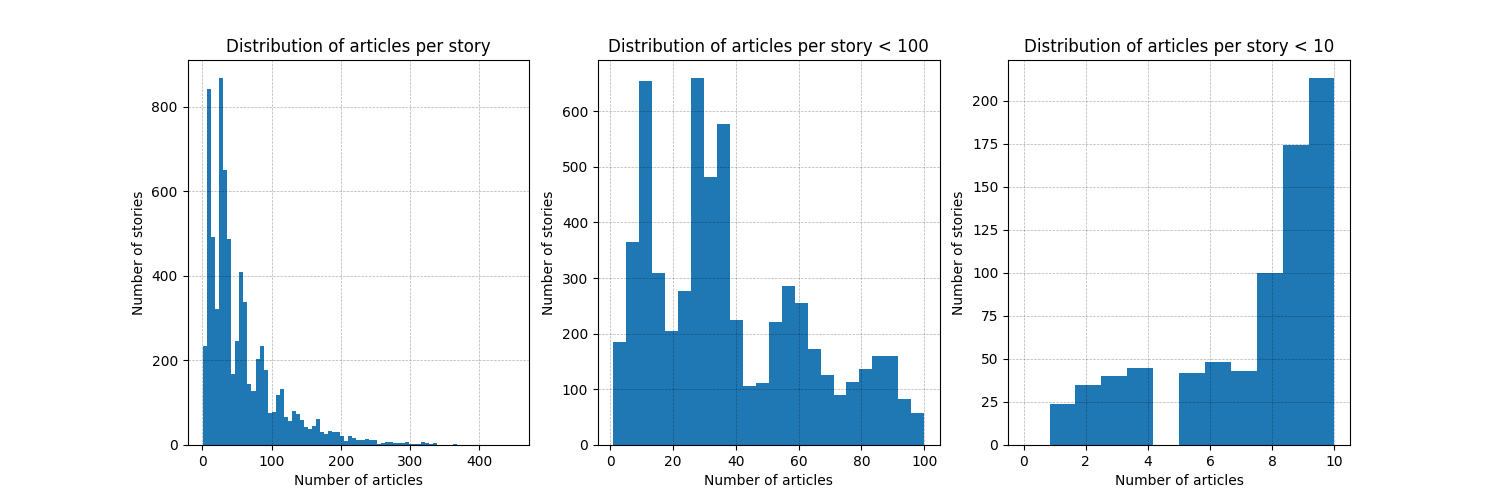
\includegraphics[width=1\textwidth]{articles_per_story_distribution}
    \caption{Distribution of cluster sizes.}
    \label{fig:articles_per_story_distribution}
\end{figure}

Focusing on the two vector space models, shows that all of the best scores per parameter have been achieved by using tf-idf.
Additionally the different metrics show a big difference when combined with word frequency.
The best scores using the word frequency are 0.071 for the euclidean metric and 0.695 for the cosine metric.
With tf-idf the difference between both metrics is still notable, but far less drastic than based on word frequency.
This can be explained by considering that the word frequency model will weigh every word equally
and therefore common words will have higher weights than less common ones.
Based on these weights, the distance calculated by the euclidean metric does not correspond well with the actual similarity between documents.
The cosine metric is less effected by these weights,
since it already calculates the similarity of two vectors instead of their distance.
Tf-idf balances out the term frequency with its inverse document frequency
and therefore less common words are weighted higher than less common ones.
As a result the euclidean distance is more effected by infrequent terms,
which are similar for similar documents and hence better scores.
Although the cosine similarity is still superior in this case.
This behaviour has already been studied in the past\cite{Strehl00impactof}\cite{similarity_measures}
and is one of the reasons, why the cosine similarity is often preferred over the euclidean distance as a similarity measure in the field of text mining.

As for the optimal preprocessing, text lemmatization provides the highest overall mp-score with 0.738,
although closely followed by text stemming.
This is to be expected, since both lemmatization and stemming reduce the dimensions by grouping words into their base form,
while still retaining most of the text.
In contrast to key term and entity extraction, which both result in a drastic reduction of the dimensions, and therefore less detail.
It is also interesting to see how close the score from using the full text is compared to the best score per row.
The difference between the overall best score of 0.738 achieved by lemmatization and the score provided by the full text of 0.731 is only 0.007.
This means text preprocessing has a lesser impact than initially expected.
However it is important to note, that we used pretrained models for key term and entity extraction.
Specifically training on a news corpus might improve the performance of both methods, but it was decided as to be out of scope for this thesis.

After determining the optimal settings for text preprocessing and vectorization,
we increase the sample sizes for our evaluation runs,
to get a deeper insight into the behaviour of HDBSCAN with larger data sets.
Figure \ref{fig:hdbscan_parameters} shows the scores achieved with different parameters over an increasingly large set of samples.
Based on this Figure we see the metric \textit{cosine} to be generally better than $euclidean$
and significantly more stable based on the range of the score and the quality of the clustering seems to decrease with larger sample sizes.

\begin{figure}[h]
    \centering
    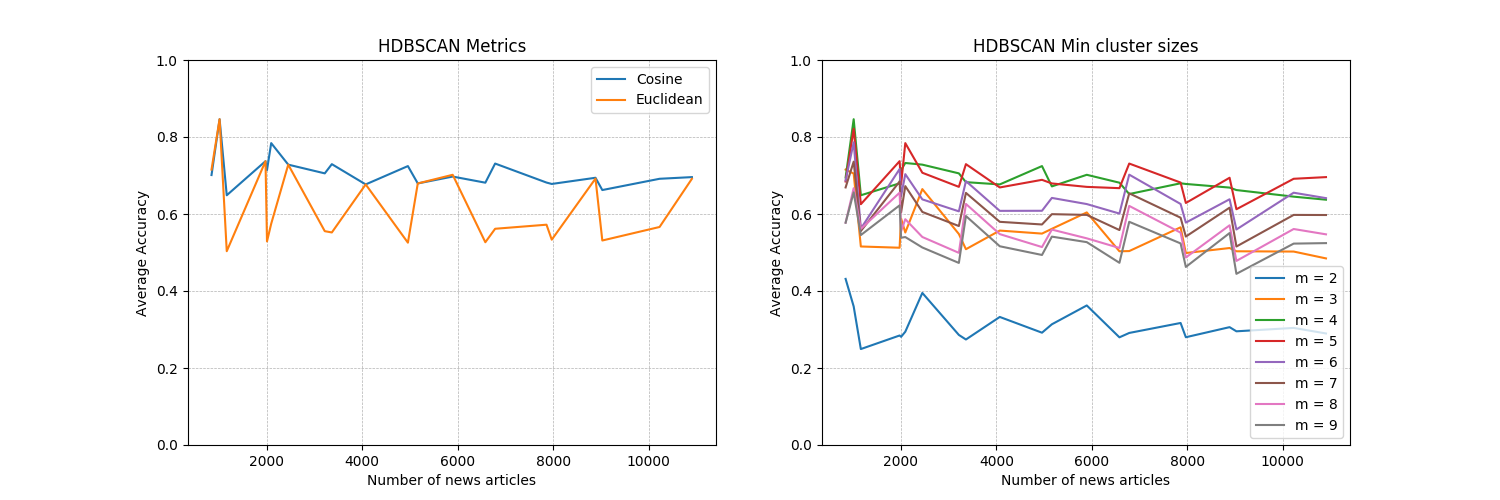
\includegraphics[width=1\textwidth]{hdbscan_parameters}
    \caption{MP-Score for different parameters, where min stands for the min cluster size. The marker represents the median, while the vertical line indicates the range between the min and max values. Each run contains at least five repetitions.}
    \label{fig:hdbscan_parameters}
\end{figure}

Furthermore the variance with smaller sample sizes can partially be explained through differences in the number of detected clusters,
since missing a few clusters has a bigger impact if the overall number of clusters is small.
Figure \label{fig:cluster_difference_samples} shows the difference between the number of predicted clusters and the number of true clusters.
The Figure provides us with an interesting observation:
While so far the minimum cluster size of six has given the best scores,
the difference in the number of clusters is much smaller with a minimum cluster size of four.
The MP-Score weights the similarity of a pair of clusters with their number of elements.
This means ignoring smaller clusters has a lesser impact than ignoring larger clusters.
We know our data set contains stories with news articles ranging from one up to 400.
Based on this knowledge and the workings of the score,
we can conclude that using a minimum cluster size of four gives us more clusters,
which are ignored by using a larger minimum cluster size, but at the same time fragmenting larger clusters.
Therefore resulting in a lower score, while having a better difference in the number of cluster predictions.
This can be validated by analysing our data directly, where we observe the number of predicted cluster to be higher the lower the minimum cluster size is.
Using $min\_cluster\_size=6$ tends to give a lower number compared the the true amount,
while $min\_cluster\_size=3$ gives usually a higher number than there are actual clusters.

\begin{figure}[h]
    \centering
    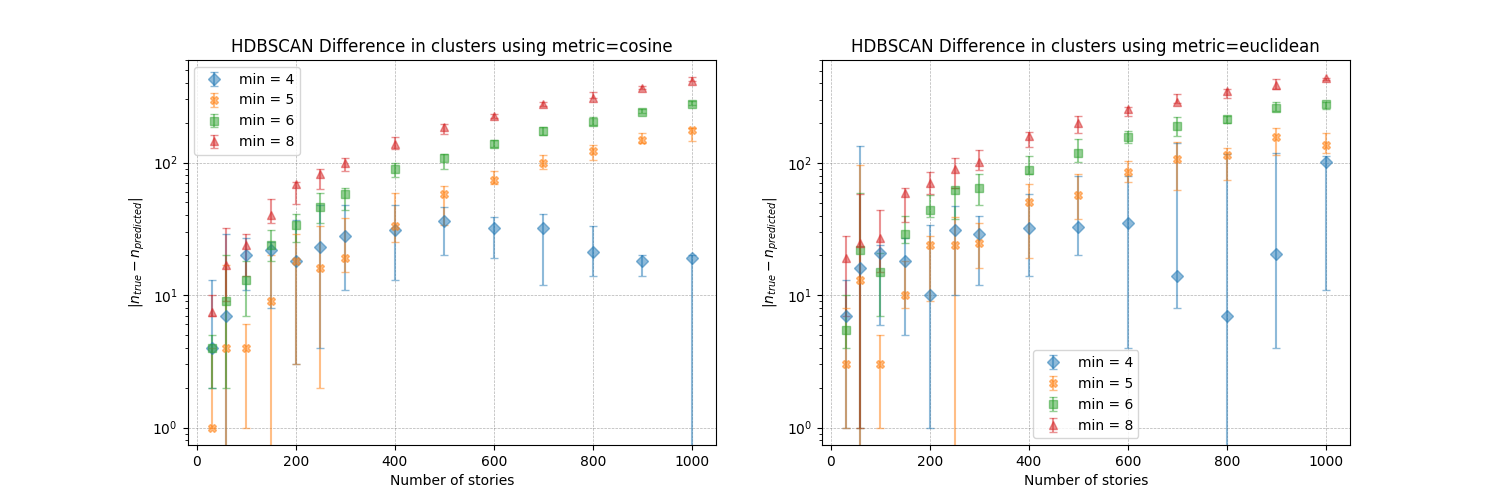
\includegraphics[width=1\textwidth]{cluster_differences}
    \caption{Difference between the predicted and true number of clusters.}
    \label{fig:cluster_differences}
\end{figure}

One of the advantages HDBSCAN has over other clustering algorithms,
is the ability to work with noise, since we intent on applying it in an online setting,
where noisy data is to be expected.
At the same time, the number of articles classified as noise should be kept to a minimum.
However the noise ratio shown in Figure \ref{fig:noise_ratio_samples} is significantly higher,
than we would expect it to be based on our test data.
A variety of factors play into the high noise ratio.
One influence is due to the $min\_cluster\_size$.
Each news article belonging to a cluster, which has less articles than the minimum cluster size, will be counted as noise.
Table \ref{tab:expected_noise} lists the calculated percentage of news articles,
which would be ignored based on different minimum cluster sizes.
Although the percentages show that the impact the minimum cluster size has on the overall noise ratio is very limited.
It is reasonably to assume, that the test data still contains a fair amount noisy data,
even after cleaning up the data to the best of our efforts.
Decreasing the noise ratio is certainly an important part in future improvements.

\begin{figure}[h]
    \centering
    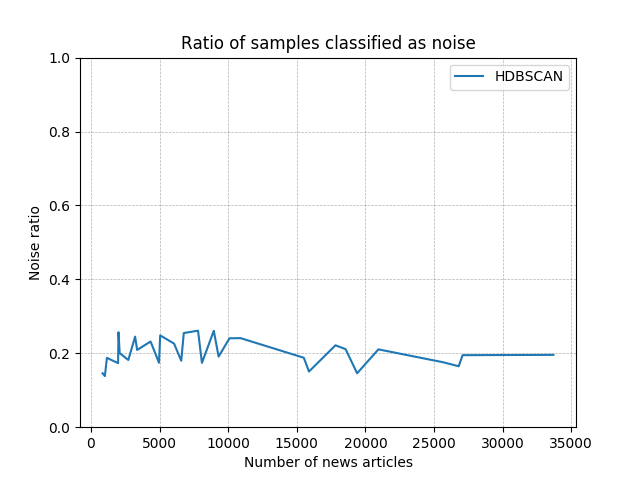
\includegraphics[width=1\textwidth]{noise_ratio_samples}
    \caption{Number of news articles classified as noise.}
    \label{fig:noise_ratio_samples}
\end{figure}

\begin{table}[h]
    \centering
    \begin{tabular}{|r|r|}
        \hline
        \textbf{min cluster size} & \textbf{Ignored articles} \\
        \hline
        2 & 0.032\% \\ \hline
        3 & 0.126\% \\ \hline
        4 & 0.304\% \\ \hline
        5 & 0.593\% \\ \hline
        6 & 0.985\% \\ \hline
        7 & 1.548\% \\ \hline
        8 & 2.168\% \\ \hline
        9 & 2.712\% \\ \hline
    \end{tabular}
    \caption{Percentages of ignored news articles because of their cluster size. The values are calculated directly based on the test data.}
    \label{tab:expected_noise}
\end{table}

Let us look closer at the data to get insights behind just the score or noise ratio.
The first story we focus on is about the hacking of U.S firms by chinese military hackers.
Table \ref{tab:clustering_example} shows a number of detected and missed news articles.
Based on the text length, we see that the missed articles are generally shorter compared with detected articles with one major exception.
Nr. 18 with a length of 13980 is nearly twice as long compared with the second longest article.
The content of Nr. 18 is a collection of different stories, only the first being about the chinese hackers.
It seems reasonable for this article to be missed in the clustering.
Articles Nr. 17, 19 and 20 all have a significantly lower length than the others,
which might already be enough to classify them as noise.
Looking at the actual contents reveals that Nr 17. is about the magazine's paywall,
Nr. 19 appears to be a short summary of the publisher itself, and Nr. 20 contains only two sentences about the topic,
a link to read more and a hint to download Acrobat Reader.
Therefore these three news articles are actual noise and ideally should have been removed during the data cleansing.
The remaining news articles appear to be valid articles about the story
and do not provide any obvious reasons for why they were regarded as noise during the clustering.

\begin{table}[h]
    \centering
    \scalebox{0.75}{

        \begin{tabular}{rlrl}
            \hline
            \multicolumn{4}{ c }{\textbf{Detected Articles}} \\
            \hline
            Nr. & Title                                                                        &   Text length & Source     \\
            \hline
                 1 & What were China's hacker spies after?                                        &          3801 & CNNMoney               \\
                 2 & Chinese Cyberespionage Crackdown Prompts Look At Intellectual Property Theft &          5124 & CRN                         \\
                 3 & FBI investigator: Many more US firms hit by Chinese military hackers         &          5585 & Tribune-Review      \\
                 4 & State-sponsored business espionage decried                                   &          3771 & Stars and Stripes          \\
                 5 & Westinghouse Among Companies in Chinese Trade Secret Hacking Case            &          1364 & Nuclear Street \\
                 6 & US charges on China hackers cap 3-year pressure drive                        &          7668 & Thanh Nien Daily        \\
                 7 & \#ShotsFired in U.S.-China Cyberwar                                           &          7352 & Daily Beast             \\
                 8 & Feds claim Chinese hackers hit US firms, including Westinghouse              &          3746 & The Cranberry Eagle       \\
                 9 & America sues China over corporate spying                                     &          4278 & Telegraph.co.uk            \\
                10 & How China's army hacked America                                              &          3427 & Ars Technica           \\
            \hline
            \\
            \hline
            \multicolumn{4}{ c }{\textbf{Missed Articles}} \\
            \hline
            Nr. & Title                                                                        &   Text length & Source                       \\
            \hline
                11 & Other views: China hacking indictments will create waves                     &          2968 & Monterey County Herald       \\
                12 & How much damage has Chinese hacking done to the US government?               &           785 & FederalNewsRadio.com         \\
                13 & FBI Releases New Details In Cyber Espionage Case                             &          2885 & CBS Local                    \\
                14 & How 5 Chinese hackers stole American companies' most closely-guarded secrets &          3726 & ITProPortal                  \\
                15 & U.S. Charges 5 Chinese Army Members with Economic Spying                     &          1093 & Democracy Now                \\
                16 & U.S. Charges Five Chinese Military Officers with Cyber Espionage             &          1823 & eSecurity Planet             \\
                17 & Prosecutors: Chinese targeted Western Pa. companies                          &           191 & Washington Observer Reporter \\
                18 & CNN's GUT CHECK for May 19, 2014                                             &         13980 & CNN                  \\
                19 & Nuclear Fallout From China's Alleged Espionage                               &           122 & Wall Street Journal \\
                20 & Charges Of Chinese Cybercrimes To Play Out In American Courts                &           443 & KPBS               \\
                \hline
        \end{tabular}
    }
    \caption{10 correctly detected and 10 missed news articles, which all belong to the same story.}
    \label{tab:clustering_example}
\end{table}

To find a possible explanation for the remaining new articles, we take a look at their tf-idf model.
Table \ref{tab:clustering_example_features} lists the top 10 keywords per news article, based on the tf-idf model.
There we see how the keywords from the detected news articles are quite similar,
while the keywords from the missing news articles appear to be more varied with minimal overlap to the keywords from detected articles.
This seems to give an indication as to why the articles were missing from the cluster.
However it is important to note, that the tf-idf model in Table \ref{tab:clustering_example_features} was created from only those 20 articles
and used the full text instead of lemmatisation for better readability.
The top keywords might differ in the model created for the whole clustering.
Especially words such as \textit{ap1000}, which is a name of a nuclear power plant, will be weighted higher in the full model.
Based on this insight we expect further work on text preprocessing to lead to considerable improvements in the quality of the clustering.

\begin{table}[h]
    \centering
    \scalebox{0.75}{
    \begin{tabular}{rl}
        \hline
        Nr. & Top 10 Keywords                                                                                                         \\
        \hline
            1 & ['chinese', 'solar', 'steel', 'power', 'firms', 'hackers', 'solarworld', 'theft', 'plants', 'ap1000']                   \\
            2 & ['theft', 'said', 'allegedly', 'data', 'security', 'businesses', 'officers', 'intellectual', 'property', 'indictment']  \\
            3 & ['said', 'companies', 'pittsburgh', 'don', 'chinese', 'company', 'security', 'accused', 'computer', 'hackers']          \\
            4 & ['said', 'companies', 'pittsburgh', 'don', 'security', 'know', 'university', 'computer', 'makes', 'chinese']            \\
            5 & ['ap1000', 'state', 'alleging', 'pipe', 'construction', 'design', 'chinese', 'westinghouse', 'china', 'owned']          \\
            6 & ['chinese', 'people', 'snowden', 'companies', 'said', 'china', 'indictment', 'evidence', 'administration', 'officials'] \\
            7 & ['chinese', 'said', 'house', 'white', 'cyber', 'department', 'indictments', 'way', 'defense', 'american']               \\
            8 & ['chinese', 'said', 'officials', 'indictment', 'company', 'mails', 'trade', 'companies', 'pennsylvania', 'stole']       \\
            9 & ['america', 'chinese', 'china', 'know', 'including', 'accused', 'targeted', 'company', 'trade', 'ap1000']               \\
            10 & ['messages', 'access', 'mail', 'according', 'indictment', 'attack', 'mails', 'spear', 'phishing', 'union']              \\
            \hline
            \hline
            11 & ['cyberspying', 'united', 'states', 'chinese', 'national', 'security', 'high', 'economic', 'aggressive', 'justice']     \\
            12 & ['report', 'world', 'cyber', 'technologies', 'economic', 'alleging', 'intended', 'links', 'programs', 'says']           \\
            13 & ['pittsburgh', 'cyber', 'allegedly', 'fbi', 'targeted', 'details', 'enforcement', 'officials', 'happens', 'threat']     \\
            14 & ['messages', 'access', 'group', 'attacks', 'like', 'mail', 'spear', 'unit', 'phishing', '61398']                        \\
            15 & ['report', 'sponsored', 'state', 'states', 'economic', 'eric', 'holder', 'case', 'united', 'intelligence']              \\
            16 & ['allegedly', 'proprietary', 'sun', '2010', 'information', 'stole', 'market', 'solarworld', 'business', 'owned']        \\
            17 & ['account', 'create', 'log', 'continue', '000', '19', '20', '2008', '2010', '2012']                                     \\
            18 & ['com', 'leading', 'don', 'obama', 'new', 'house', 'oregon', 'years', 'people', 'state']                                \\
            19 & ['news', 'leading', 'media', 'corp', 'network', 'information', 'companies', '000', '19', '20']                          \\
            20 & ['alleging', 'order', 'pdf', '2014', 'alleges', 'filed', 'firms', 'chinese', 'documents', 'hacked']                     \\
        \hline
        \end{tabular}
        }
        \caption{Top 10 keywords extracted from the tf-idf model.}
        \label{tab:clustering_example_features}
\end{table}

So far we focused on HDBSCAN to determine the optimal settings to run it with.
As a next step we can start comparing the overall performance with \textit{k}-means.
We use the follwing settings: Text lemmatisation with tf-idf,
cosine as the similarity measure and six as the minimum size of clusters.
Figure \ref{fig:precision_and_processing_time_kmeans_hdbscan} shows a similar behaviour
for both clustering methods in value and variance of the precision.
Although HDBSCAN is generally more accurate than \textit{k}-means,
the difference gets smaller with an increase in the sample size.
Additionally the increase in the number of samples results for both HDBSCAN
and \textit{k}-means in a small loss regarding the precision as can be seen in Figure \ref{fig:precision_and_processing_time_kmeans_hdbscan}
and which we have already observed when analysing HDBSCAN parameters.

\begin{figure}[h]
    \centering
    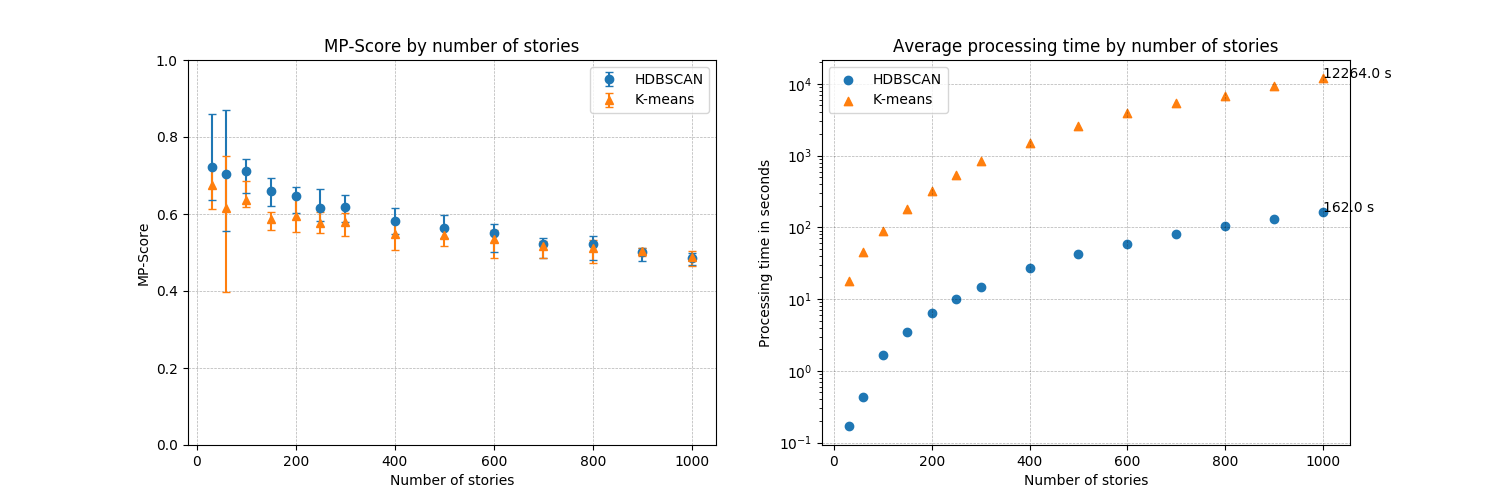
\includegraphics[width=1\textwidth]{accuracy_and_processing_time_kmeans_hdbscan}
    \caption{Comparison of the MP-Score and processing time between \textit{k}-means and HDBSCAN}
    \label{fig:precision_and_processing_time_kmeans_hdbscan}
\end{figure}

While HDBSCAN and \textit{k}-means provide a similar score,
the biggest difference can be noted in the processing time in relation to the number of samples.
\textit{k}-means has a time complexity of $O(n^2)$ in contrast to HDBSCAN with a time complexity of $O(nlog(n))$,
which is illustrated by Figure \ref{fig:precision_and_processing_time_kmeans_hdbscan}.
Although running the evaluation has also shown the space complexity for HDBSCAN
to be substantially higher for larger amounts of samples than with \textit{k}-means.
Trying to run HDBSCAN with 100'000 news articles caused in a memory error,
even with 64GB of RAM, while \textit{k}-means was able to complete the clustering.
The memory issue with large data sets is known and according to the author the current implementation of HDBSCAN
is not optimised for memory\cite{hdbscan_memory_issue}.
This might be another area for further improvements, although it will not help to increase the score on larger data sets.

As a final evaluation, we compare HDBSCAN with six different clustering methods taken from scikit-learn.
Each method is run with a variety of parameters and the best scores are shown in Figure \ref{fig:different_clusterings}.
HDBSCAN provides the highest precision, while being still being one of the fastest algorithms.
We are aware of our bias for HDBSCAN since we invested a significant amount understanding and analysing it,
but it is still interesting to see how well it compares with other clustering methods out of the box.

\begin{figure}[h]
    \centering
    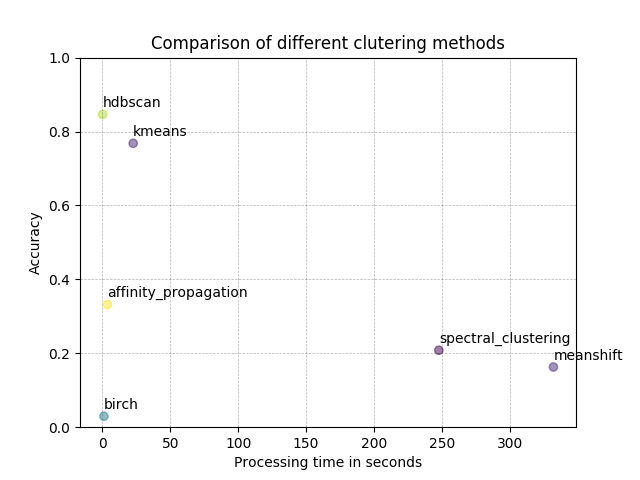
\includegraphics[width=0.5\textwidth]{different_clusterings}
    \caption{Comparison of different clustering methods with a sample size of approximately 1000 news articles}
    \label{fig:different_clusterings}
\end{figure}

\subsubsection{Conclusion}
\label{subsubsec:5a_conclusion}

The evaluation has shown HDBSCAN to be a good candidate to use for text based clustering.
It provides an better precision than \textit{k}-means, while being significantly faster to process.
The predicted number of clusters is consistent with an increasing number of samples and fairly close the truth.
Additionally we have shown the required preprocessing and vectorization steps with the ideal parameters to achieve the most accurate results for our data set.
However there is a substantial noise ratio, which causes almost a third of the processed samples to be classified as noise.
We have also analysed individual clusters and discovered,
that the vector space model can vary substantially between news articles of the same cluster.
Another consideration is the space complexity with larger data sets,
where we quickly ran into issues when clustering high number of samples.
Overall HDBSCAN provides an acceptable precision, while still leaving room for further improvements.
